\chapter{Классификация существующих решений}
В данном разделе представлены существующие идеи, заложенные в основе параллельного логического программирования, и описан предложенный способ реализации на графическом процессоре.

\section{Использование неявного параллелизма}
Фундаментальная идея, лежащая в основе неявного параллелизма, основывается на том, чтобы сделать его прозрачным для программиста, автоматически выполняя параллельно некоторые шаги, относящиеся к операционной семантике языка \cite{parallel_logic}.

\subsection{AND-параллелизм}
Оригинальные реализации независимого AND-параллелизма основывались на низкоуровневых действиях с базовой машиной -- служит вариантом расширения абстрактной машины Уоррена \cite{warren}. Такой низкоуровневый подход необходим для снижения накладных расходов на выполнение, связанное с параллелизмом; но эти реализации довольно трудно поддерживать с улучшением технологии последовательного выполнения.

Методы зависимого AND-параллелизма нашли применение в системах логического программирования, которые развились из Prolog, таких как Mercury  \cite{mercury} и EAM (Extended Andorra Model) \cite{eam}.

Упрощенную архитектуру для зависимого AND-параллелизма можно найти в параллельной реализации \textit{Mercury} \cite{mercury_new}. Предлагаемая архитектура использует многопоточную реализацию для создания нескольких <<рабочих>>, которые одновременно выполняют некоторые подцели. Позже это было расширено до реализации, которая поддерживает связь между подцелями. Предложенная система заменяет использование единой централизованной очереди задач набором локальных рабочих очередей, аналогичным иным AND-параллельным реализациям Пролога. Другим компонентом этой системы является использование анализа затрат для выявления перспективных подцелей во время компиляции для параллельного выполнения.

\textit{EAM}. Расширенная модель Андорры позволяет выполнять подцели одновременно до тех пор, пока они детерминированы или пока они не запрашивают недетерминированную привязку внешней переменной. Когда присутствует недетерминизм, вычисление может разделиться в форме OR-параллелизма


\subsection{OR-параллелизм}
С. Коста, И. Дутра предложили реализацию OR-параллелизма в многопоточной версии YAP Prolog \cite{costa}, которая опирается на модель копирования стека. Позже совместно с Р. Роша они распространили этот подход на системы, состоящие из кластеров многоядерных процессоров, решая проблему сочетания архитектур общей и распределенной памяти \cite{rosha}. Ими была предложена многоуровневая модель, основанная на два уровня <<работников>>: <<одиночные работники>> и <<группы работников>>, а также возможность использовать различные стратегии планирования для распределения работы между командами и между <<работниками>> внутри команды. Команда <<работников>> формируется теми <<работниками>>, которые совместно используют одно и то же адресное пространство памяти.
 
\section{Использование GPU}
Графические процессоры (GPU) --- это устройства с параллельной структурой, изначально разработанные для поддержки компьютерной графики и обработки изображений. В последнее время использование таких многоядерных систем стало широко распространенным в приложениях, которые требуют объемных вычислительных мощностей. Архитектура GPU отличается от CPU (рисунок \ref{image:cpu_vs_gpu}).

\begin{figure}[H]
	\centering{
		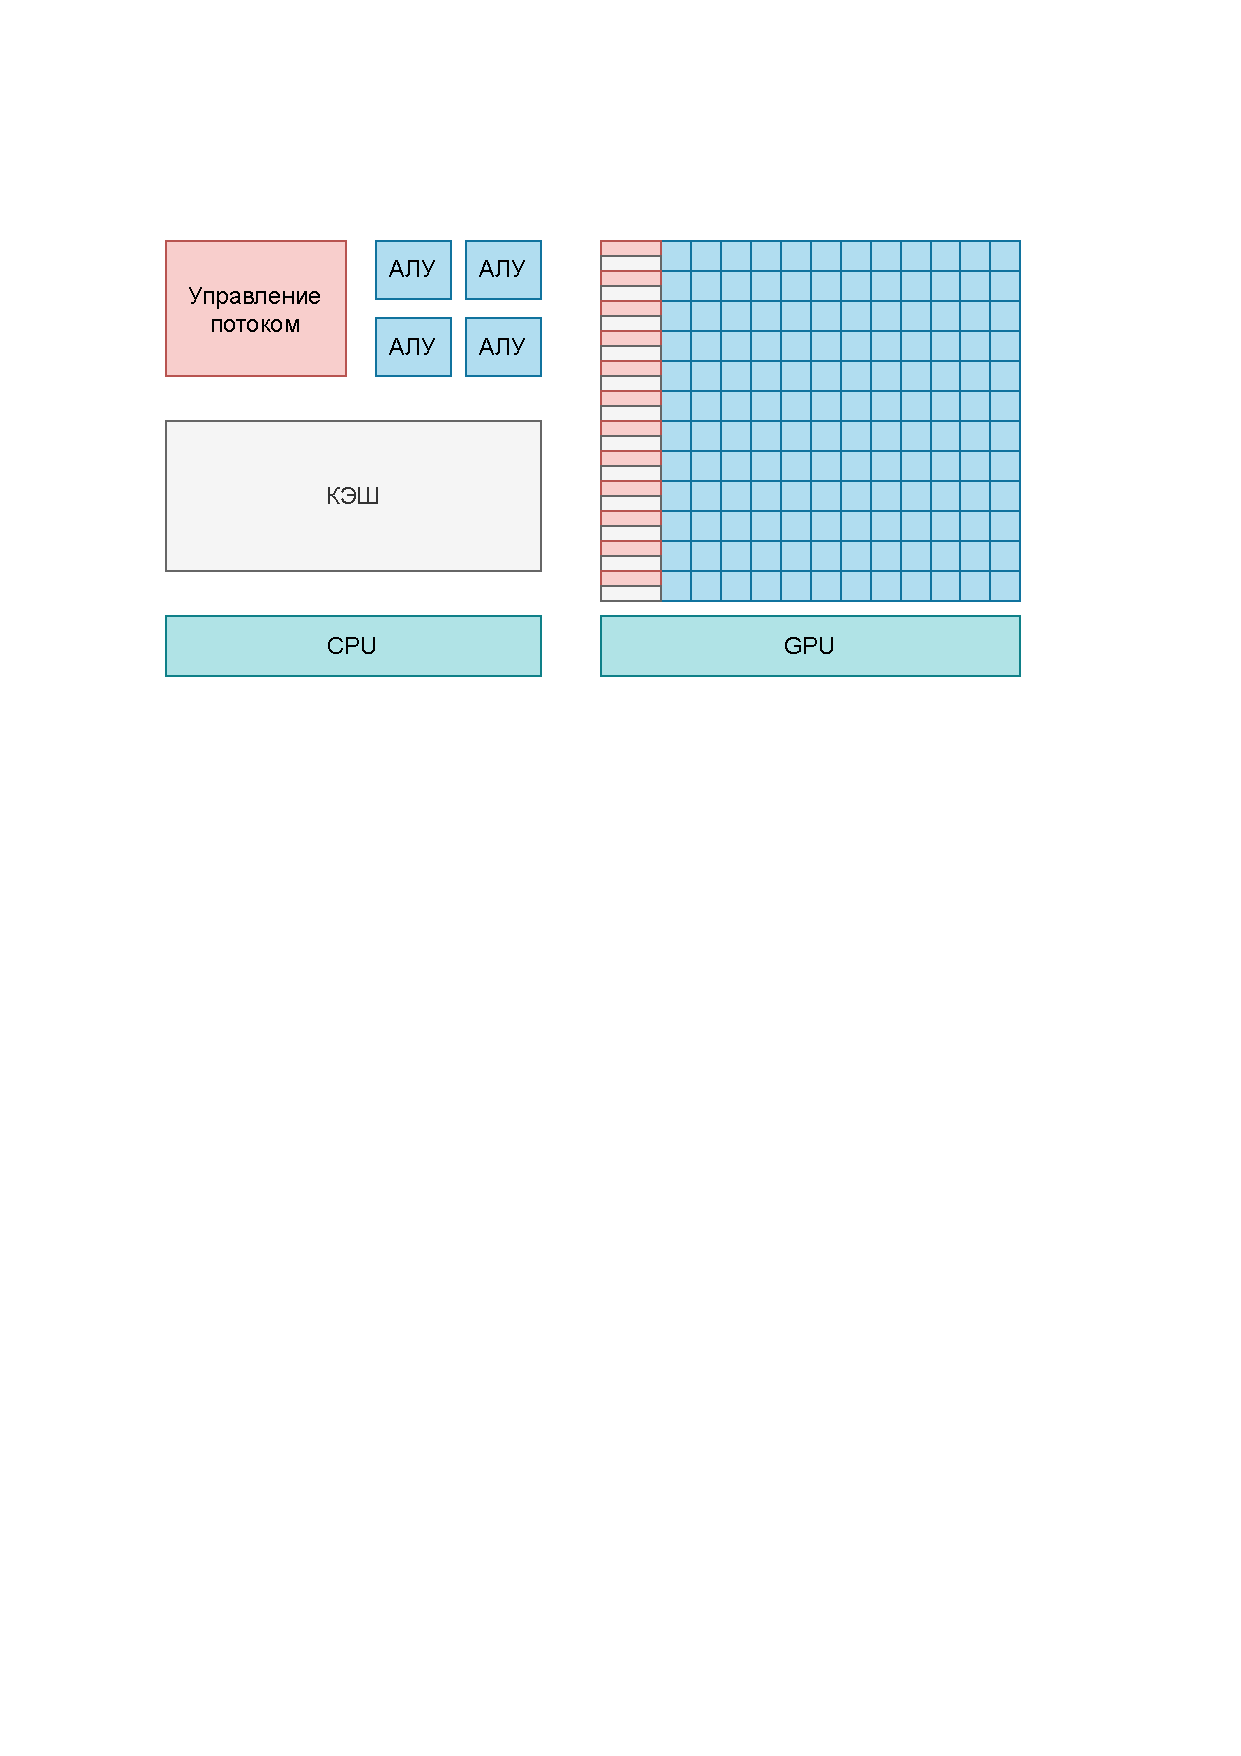
\includegraphics[scale=1]{images/cpu_vs_gpu.pdf}
		\caption{Различие между архитектурами CPU и GPU.}
		\label{image:cpu_vs_gpu}}
\end{figure} 

\subsection{Программное обеспечение для работы с GPU}
Для работы с графическими процессорами существует несколько распространенных технологий.

\begin{enumerate}
	\item CUDA. Данная технология предназначена для разработки приложений на массивно-параллельных вычислительных устройствах. Архитектура построена так, что GPU выступает в качестве сопроцессора для CPU \cite{cuda}.	Вычисления организованы в виде сетки блоков потоков; внутри каждого блока потоки выполняются одновременно, но на остальных блоках они могут находиться на разных стадиях выполнения. Таким образом, каждая подзадача решается отдельно. Число одновременных выполняемых потоков зависит от числа ядер на графическом процессоре. В современных устройствах оно отличается от числа центрального процессора в большую сторону. Так NVIDIA TITAN X (PASCAL) содержит 3584 ядер \cite{nvidia_titan_x}, что позволит ускорить время выполнения задач.	
	
	\item OpenCL. Модель платформы состоит из хоста, подключенного к одному или нескольким устройствам OpenCL; каждое из них разделено на один или несколько вычислительных блоков, которые далее также разделены на один или несколько элементов обработки \cite{opencl}, внутри которых выполняются вычисления на устройстве. Предоставляется иерархическая модель параллельного программирования данных. Существует два способа указать иерархическое подразделение. В явной модели определяется общее количество рабочих элементов для параллельного выполнения, а также то, как рабочие элементы распределяются между рабочими группами. В неявной модели указывается только общее количество рабочих элементов для параллельного выполнения, а разделение на рабочие группы управляется реализацией OpenCL.
\end{enumerate}


\section{Движок Datalog на GPU}
Программы Datalog могут быть оценены при помощи подходов <<сверху-вниз>> и <<снизу-вверх>>. В первом начинает выполнение с цели и сводится к подцелям до тех пор, пока простое решение не будет найдено. Такой подход, использующийся в Prolog, не может быть выполнен на GPU ввиду того, что время обработки отдельных кортежей может отличаться в разы.

Во втором подходе применяются правила к данным фактам, тем самым выводятся новые; Этот процесс повторяется до тех пор, пока больше не будет ничего получено. Запрос рассматривается только в конце для выбора нужных факты, которые ему соответствуют. Этот подход подходит для GPU, поскольку такие реляционные операции показывают одинаковое время обработки для разных кортежей. Также правила могут оцениваться в любом порядке.

GPU-Datalog основан на трех основных операторах реляционной алгебры: select, join, projection \cite{gpu_datalog}. Это представлено на рисунке \ref{image:evaluation_based_datalog}.

\begin{figure}[H]
	\centering{
		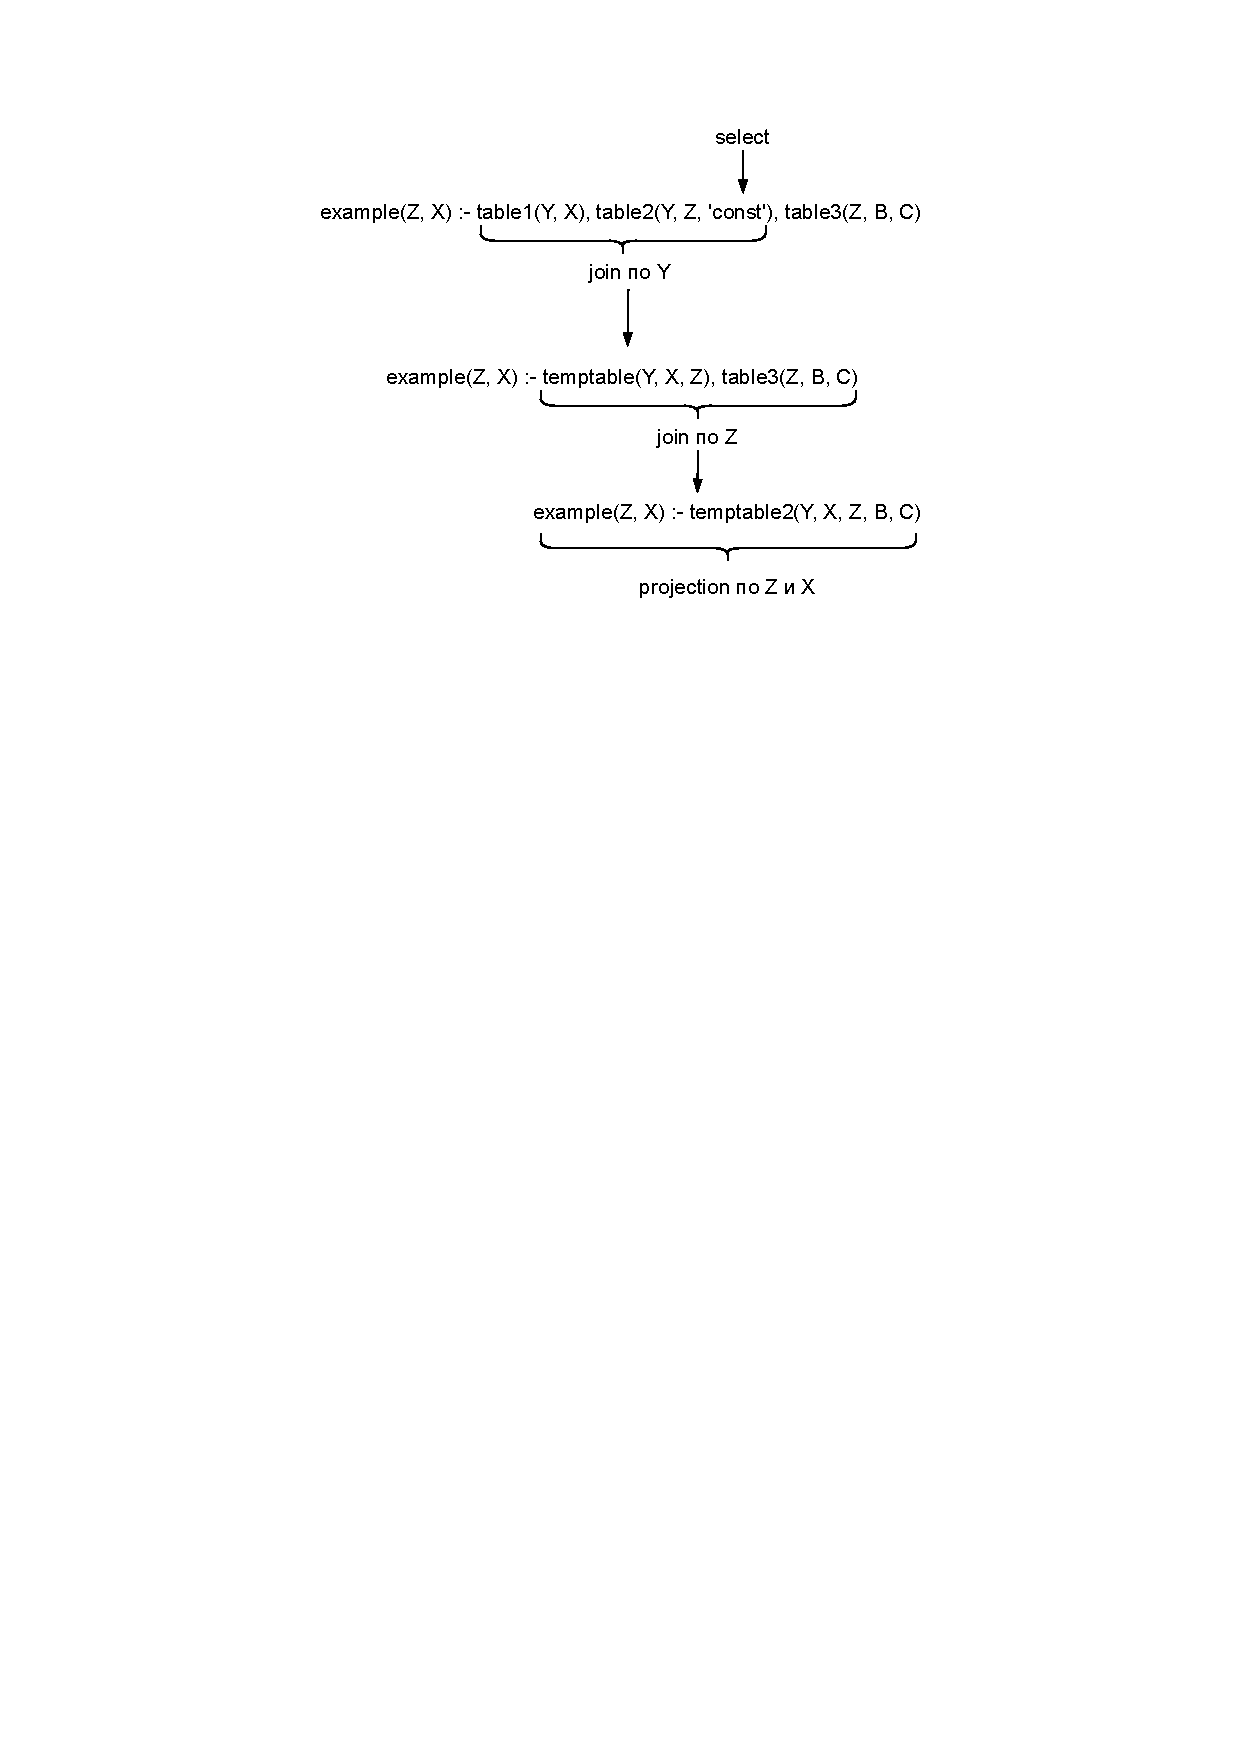
\includegraphics[scale=1]{images/compulation_base.pdf}
		\caption{Оценка Datalog на основе операций реляционной алгебры.}
		\label{image:evaluation_based_datalog}}
\end{figure} 

GPU-Datalog также включает вторичные операторы как отрицание (¬), сравнение (<, >, <, =, >=, <=), агрегатную функцию (GROUP BY) и связанные с ним операции (SUM, COUNT, AVG) и арифметические знаки \newline (+, -, *, /))

GPU-Datalog был интегрирован в качестве модуля в YAP Prolog \cite{yap_prolog}, чтобы связать модель базы данных с миром графических процессоров. Представляет собой комплексное решение, в котором используются как GPU, так и CPU. Движок этой реализации организован при помощи различных ядер GPU. При раскрытии правила для каждой пары подцелей сначала выбираются ядра select и selfjoin для устранения нерелевантных кортежей. За ними следуют другие ядра - join и projection. При этом данные, посылаемые на GPU, организованны в виде массивов, хранящихся в глобальной памяти.

Чтобы использовать возможности графического процессора для обработки чисел и иметь минимальное возможное время обработки каждого кортежа, факты и правила идентифицируются с числами и используются как числа. Таким образом, строки хранятся в хэшированном словаре, где уникальной строке присваивается уникальный номер. 


\textit{Выборка (select)}: определяется двумя значениями (номер столбца и значение константы), которые посылаются  массив, хранящий более чем одну выборку. Например, столбцы с номерами 0, 2, 5 будут определять константы a,b,c соответственно (формула (\ref{eq:formula_1})).

\begin{equation}
	\label{eq:formula_1}
	fact1('a', X, 'b', Y, Z, 'c'). \rightarrow [0, 'a', 2, 'b', 5, 'c']
\end{equation}


\textit{Соединение (join)}: определяется двумя значениями - номер столбца по отношению к первому соединению и номером столбца по отношению ко второму соединению (формула (\ref{eq:formula_2})):

\begin{equation}
	\label{eq:formula_2}
	fact1(A, X, Y, Z), fact2(Z, X, B, C, Y). \rightarrow [1, 1, 2, 4, 3, 0]
\end{equation}


Другие операции организованы также с использованием массивов чисел, которые хранятся в разделяемой памяти GPU ввиду их малого размера.

\subsection{Распределение памяти на GPU}
Передача данных между памятью графического процессора и памятью хоста (CPU) является дорогостоящей. Предложена схема управления памятью, которая пытается свести к минимуму количество таких передач \cite{gpu_datalog}. Её цель состоит в том, чтобы сохранять факты и результаты правил в памяти графического процессора как можно дольше, чтобы, если они используются более одного раза, их можно было часто повторно использовать из памяти графического процессора. Для этого отслеживается доступная и используемая память графического процессора, а также ведется список с информацией о каждом факте и результате правила, которые хранятся в памяти графического процессора. Когда данные (факты или результаты правил) запрашиваются для загрузки в память графического процессора, они сначала
просматриваются в этом списке. Если он найден, его запись в списке перемещается в начало списка; в противном случае для данных выделяется память, и для них создается запись списка в начале списка. В любом случае возвращается его адрес в памяти . Если для выделения памяти для данных требуется освободить другие факты и результаты правил, сначала освобождаются те, которые находятся в конце списка, до тех пор, пока не будет получено достаточно памяти — результаты правил записываются в память процессора перед их освобождением. Таким образом, результаты последних использованных фактов и правил сохраняются в памяти графического процессора.

\subsection{Операторы реляционной алгебры на GPU}
Выборка (select): для запуска на GPU необходимо возникают следующие моменты:

\begin{enumerate}
	\item результат выборки предварительно неизвестен;
	\item каждый поток графического процессора должен знать, в какую ячейку глобальной памяти он запишет свой результат, не связываясь с другими потоками графического процессора.
\end{enumerate}

Для решения этих проблем используются три разных ядра: первое помечает все строки, удовлетворяющие предикату выбора; второе выполняет суммирование префиксов для меток, чтобы определить размер буфера результатов и местоположение. Последнее --- записывает полученные результаты.

Соединение (join): используются три типа соединения - одиночное (необходимо для соединения двух столбцов $table_1(X, Y)$ и $table_2(Y, Z))$, множественное (соединение двух и более столбцов - $table_1(X,Y)$ и $table_2(X,Y)$), самообъединение (соединение двух одинаковых столбцов той же таблицы $table_1(X,X)$). Улучшение версии Indexed Nested Loop Join включает CSS-дерево (Cache Sensitive Search Tree - дерево поиска с учетом кэша). Такая структура очень подходит для графических процессоров, поскольку её можно построить параллельно.

Проекция (projection): включает в себя взятие всех элементов каждого требуемого столбца и сохранение их в новой ячейке памяти. Более высокая пропускная способность памяти графического процессора по сравнению с пропускной способностью центрального процессора и тот факт, что результаты остаются в ней графического процессора для дальнейшей обработки, делают проекцию подходящей операцией для обработки на графическом процессоре.

\subsection{Экспериментальная оценка}
На рисунках \ref{image:graphic_1} и \ref{image:graphic_2} представлены результаты эксперимента по сравнению скорости выполнения реализации GPU-Datalog и YAP-Prolog \cite{datalog}.

\begin{figure}[H]
	\centering{
		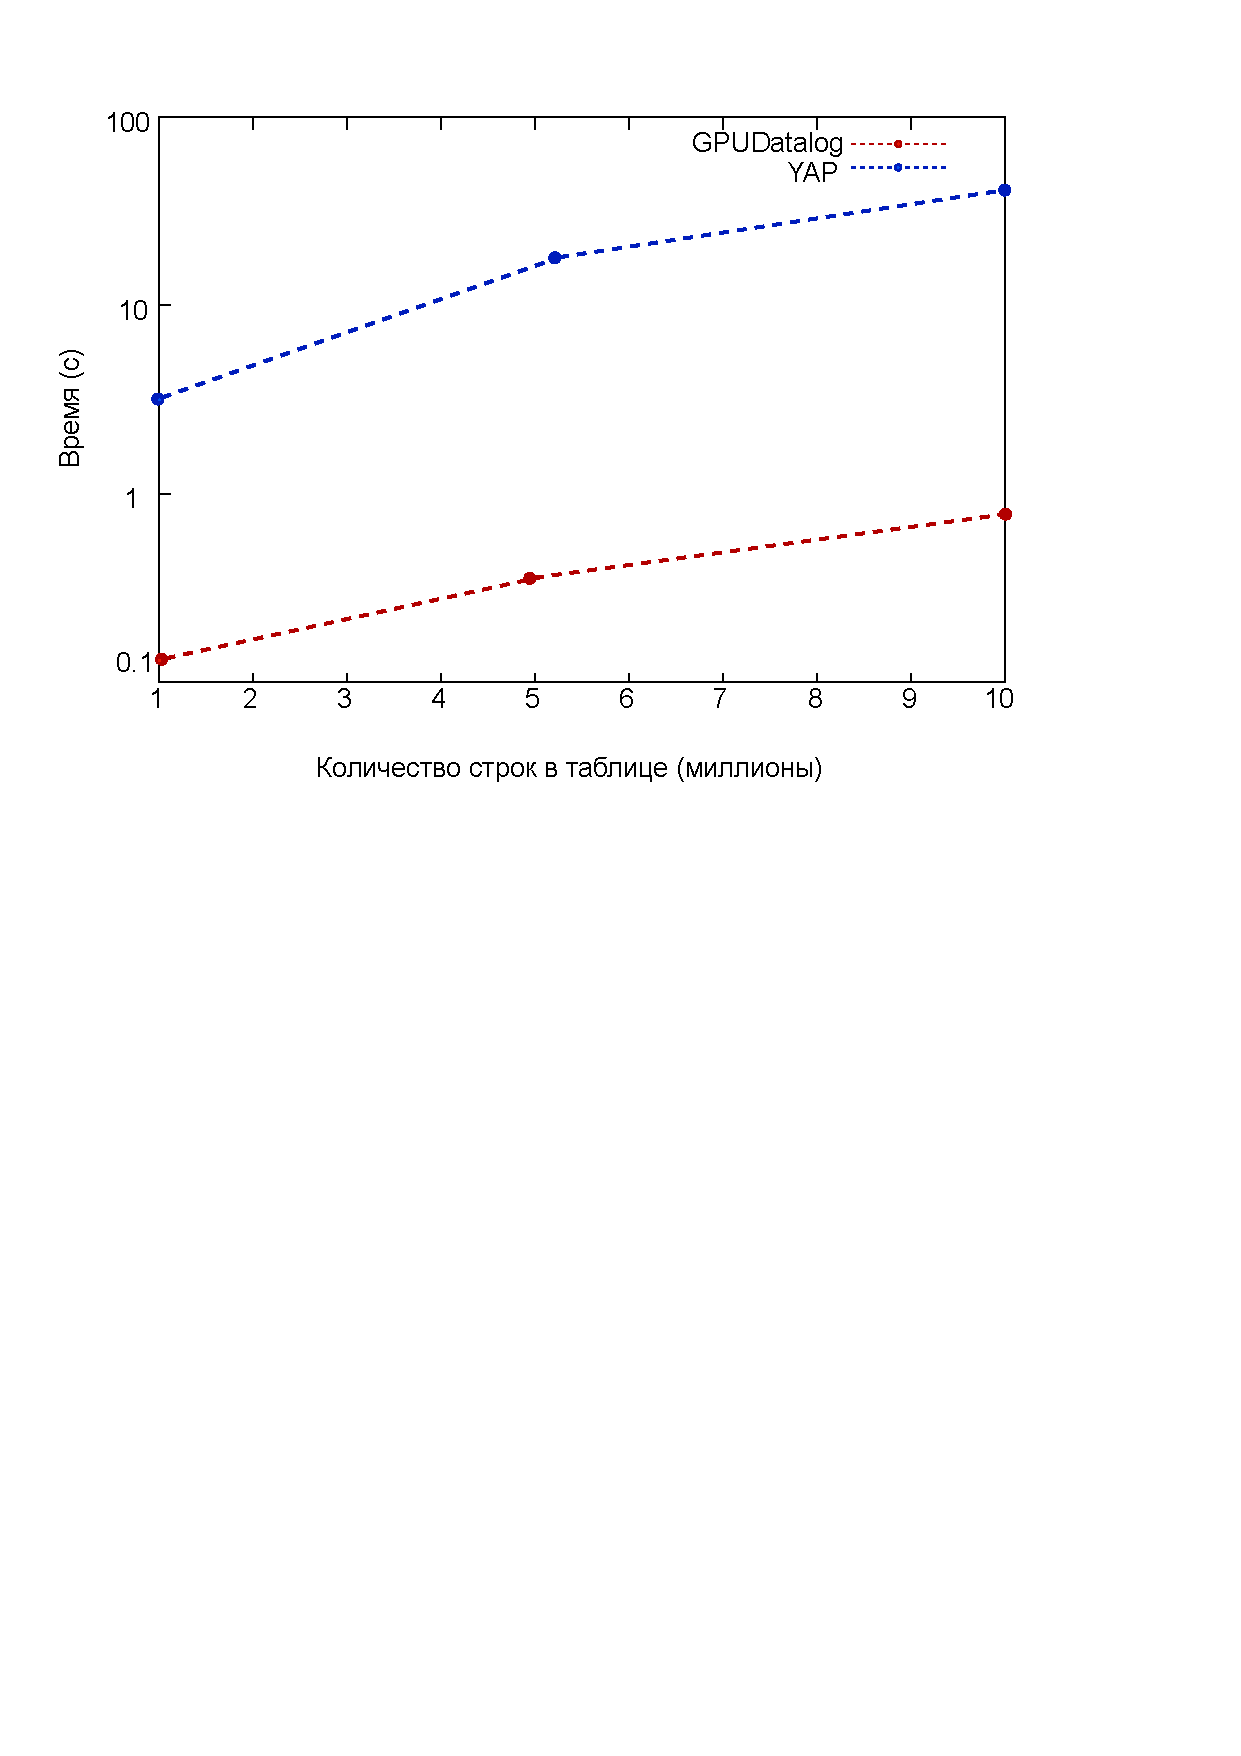
\includegraphics[scale=0.8]{images/graphic_1.pdf}
		\caption{Выполнение операции join.}
		\label{image:graphic_1}}
\end{figure} 

\begin{figure}[H]
	\centering{
		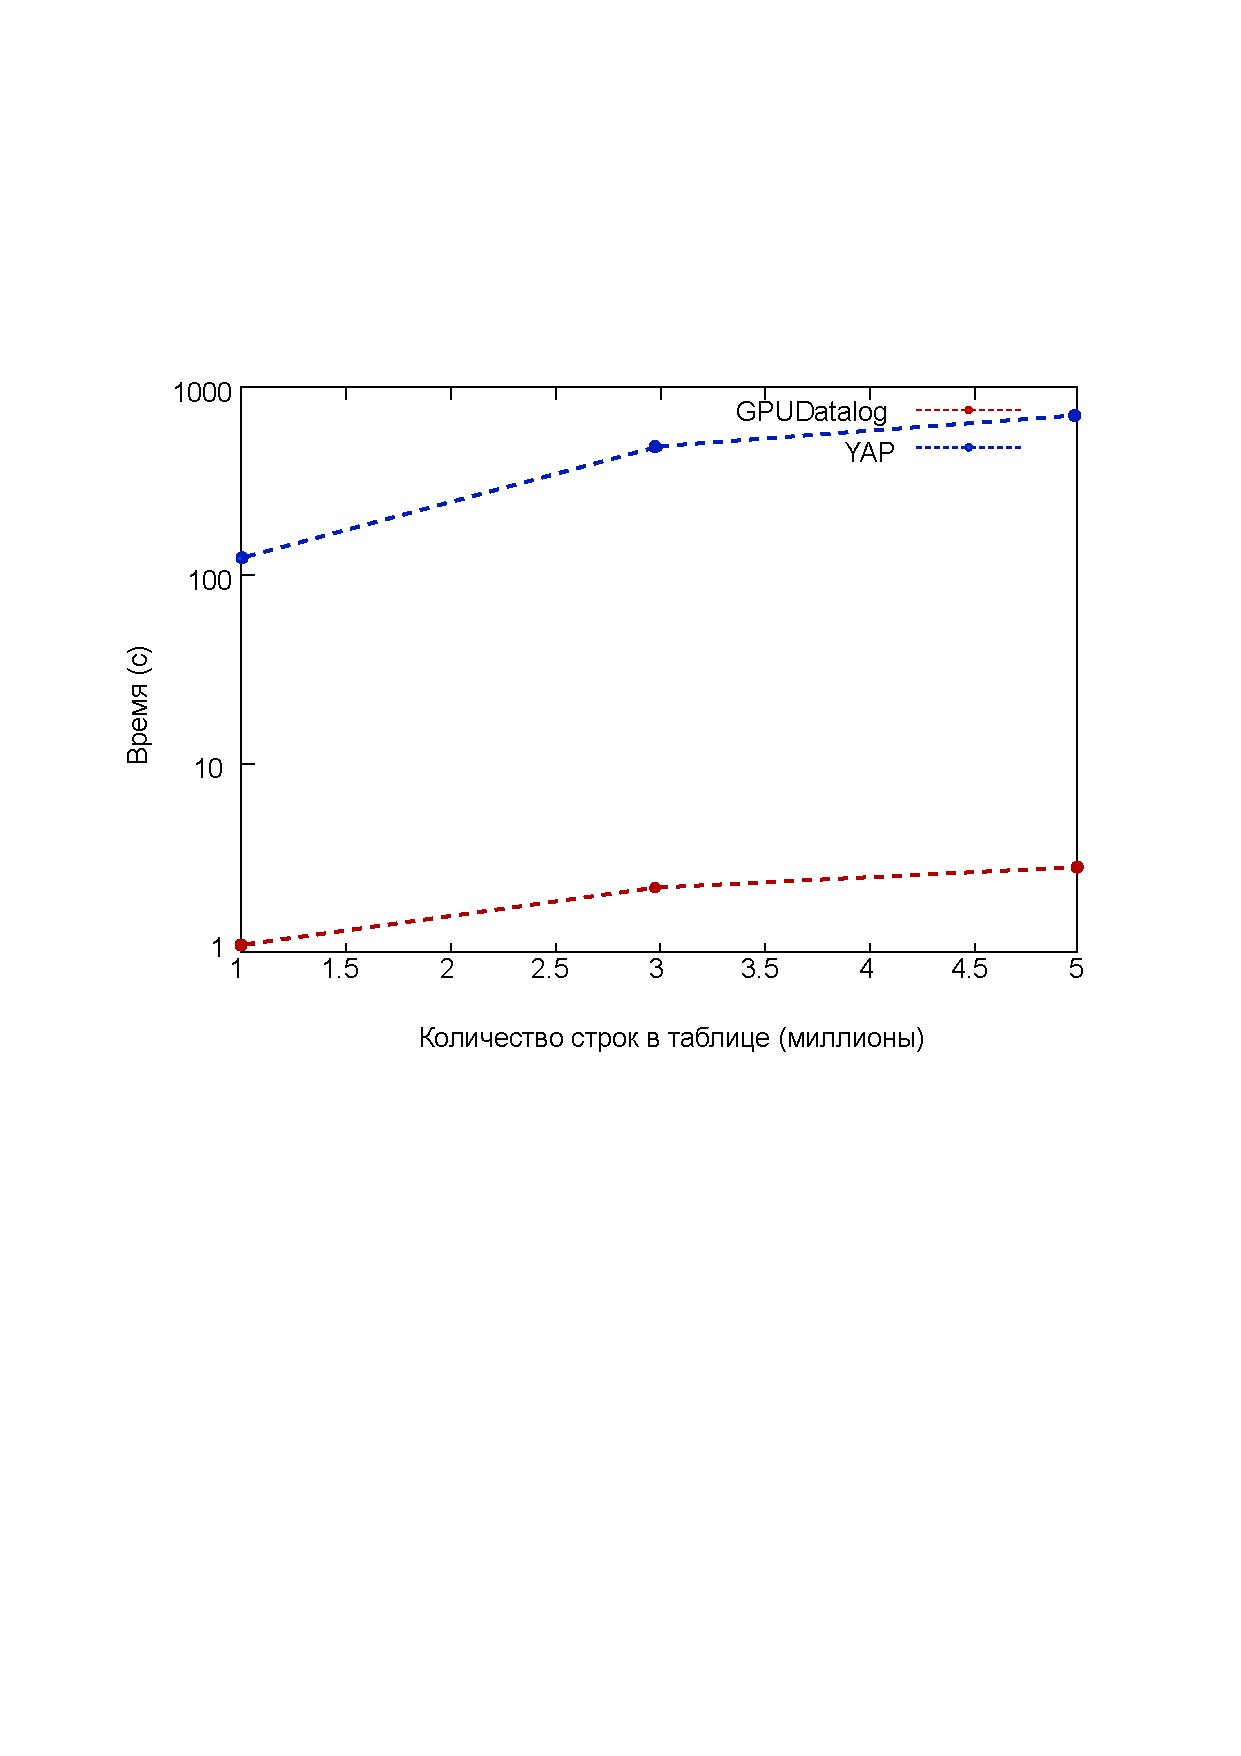
\includegraphics[scale=0.8]{images/graphic_2.pdf}
		\caption{Выполнение рекурсивного запроса.}
		\label{image:graphic_2}}
\end{figure} 

Приведенные результаты представляют перспективным направление развития GPU-Datalog на основе Prolog и расширенных инструкций WAM.

\section{Вывод}
Подход к распараллеливанию логического вывода формировался в разных представлениях. Стали развиваться идеи реализации на графических процессорах ввиду их быстродействия по сравнению с CPU \cite{fast_gpu_over_cpu}. 